%%%%%%%%%%%%%%%%%%%%%%%%%%%%%%%%%%%%%%%%%%%%%%%%%%%%%%%%%%%%%%%%%%%%%%%%%%%%%%%
% Definición del tipo de documento.                                           %
% Posibles tipos de papel: a4paper, letterpaper, legalpapper                  %
% Posibles tamaños de letra: 10pt, 11pt, 12pt                                 %
% Posibles clases de documentos: article, report, book, slides                %
%%%%%%%%%%%%%%%%%%%%%%%%%%%%%%%%%%%%%%%%%%%%%%%%%%%%%%%%%%%%%%%%%%%%%%%%%%%%%%%
\documentclass[11pt, spanish, a4paper]{article}

%%%%%%%%%%%%%%%%%%%%%%%%%%%%%%%%%%%%%%%%%%%%%%%%%%%%%%%%%%%%%%%%%%%%%%%%%%%%%%%
% Los paquetes permiten ampliar las capacidades de LaTeX.                     %
%%%%%%%%%%%%%%%%%%%%%%%%%%%%%%%%%%%%%%%%%%%%%%%%%%%%%%%%%%%%%%%%%%%%%%%%%%%%%%%
\usepackage[spanish]{babel}     % Paquete para definir el idioma usado.
\usepackage[latin1]{inputenc}   % Define la codificaci�n de caracteres 
                                % (latin1 es ISO 8859-1)
%\usepackage[T1]{fontenc}        % Agrega caracteres extendidos al font
\usepackage{t1enc}
\usepackage{palatino}           % Cambia el font por omision a Palatino
\usepackage{graphicx}           % Paquete para inclusi�n de gr�ficos.
%%%%%%%%%%%%%%%%%%%%%%%%%%%%%%%%%%%%%%%%%%%%%%%%%%%%%%%%%%%%%%%%%%%%%%%%%%%%%%%

% T��tulo principal del documento.
\title{\textbf{The Speaker (Trabajo Pr�ctico Nro. 1)}}

% Informaci�n sobre los autores.
\author{    
            Juan Manuel Barrenche, \textit{Padr�n Nro. 86.152}               \\
            \texttt{ snipperme@gmail.com }                                   \\
            Mart��n Fern�ndez, \textit{Padr�n Nro. 88.171}                    \\
            \texttt{ tinchof@gmail.com }                                     \\
            Ra�l Lopez, \textit{Padr�n Nro. 88.430}                           \\
            \texttt{ rau\_carpo@hotmail.com }                                \\
            Marcos J. Medrano, \textit{Padr�n Nro. 86.729}                   \\
            \texttt{ marcosmedrano0@gmail.com }                              \\
            Federico Valido, \textit{Padr�n Nro. 82.490}                     \\
            \texttt{ fvalido@gmail.com }                                     \\ 
                                                                             \\
            \normalsize{Grupo Nro. 11 (YES) - 1er. Cuatrimestre de 2009}     \\
            \normalsize{75.06 Organizaci�n de Datos}                         \\
            \normalsize{Facultad de Ingenier�a, Universidad de Buenos Aires} \\
       }
\date{Domingo 5 de Abril de 2009}


% Comienzo del documento
\begin{document}

\maketitle                % Inserta el t�tulo.
\thispagestyle{empty}     % Quita el n�mero en la primer p�gina.

% Resumen que aparece en la primera p�gina (antes de la tabla de contenidos)
\begin{abstract}
Este parrafo deber�a contener una breve descripci�n del trabajo practico. No 
deber�a contener mas de 100 palabras.
En una introducci�n posterior se podr�a describir con m�s detalle los contenidos
de este trabajo.
Documento desarrollado en LATEX.
\end{abstract}

\newpage
\tableofcontents        % Comentar si no se desea la Table Of Content.
\newpage

% Inclusi�n de archivos externos
\section{Introducci�n}

texto
         % Introducci�n
\section{Arquitectura del Sistema}

texto

\subsection{Subsecci�n}

texto

\subsubsection{SubSubSecci�n}

texto
          % Descripci�n general de la Arquitectura e introducci�n de cada Modulo
\section{Manejadores de Archivo}

Los datos que manejara **The Speaker** ten�an, como requerimiento t�cnico, que ser persistidos en dos archivos separados y deb�an utilizar la siguiente estructura l�gica.
\begin{enumerate}
	\item \texttt{((palabra)i, offset)}
	\item \texttt{(stream de audio)}
\end{enumerate}
El primero est� compuesto de la dupla palabra (que es un identificador) y offset/referencia. Simbolizando que para la {\it palabra} el audio se encuentra en {\it referencia}.
El segundo archivo contiene los streams de audio capturados.

\subsection{An�lisis}
Lo primero que se observa de ambos archivos es que sus registros son de longitud variable y que hay homogeneidad en los datos a almacenar, es decir, que en cada archivo se almacenan siempre los mismos tipos de datos. De manera que, ambos archivos, a pesar de tener naturalezas de datos diferentes requieren el mismo manejo. Por lo cual, admiten una misma soluci�n de manejo del archivo mientras que la misma se mantenga indepen de la naturaleza de los datos a almacenar. 

Por otra parte, las operaciones que se deben permitir son el agregado de registros y la consulta de los mismos. El agregado de registros no requiere, en ninguno de los dos casos, que se haga con un orden espec�fico. Mientras que la recuperaci�n de los datos, por otra parte, en el primer archivo debe poder ser secuencial (ya que se necesitan poder acceder a cada una de las palabras) y en el segundo caso debe poder accederse directamente a un registro que conozco su posici�n dentro del archivo. Por lo cual, estamos ante una organizaci�n secuencial de acceso relativo. Pudiendo recorrerse tanto secuencialmente como acceder a un registro espec�fico (si se conoce previamente su direcci�n).

\subsection{Soluci�n propuesta}
\paragraph{}
Se utilizar�n instancias de una clase llamada \textbf{VariableLengthFileManager} para abstraer a cada uno de los archivo. Esta clase define el comportamiento tanto, de la carga de registros, como de las dos formas diferentes de recuperaci�n de registros (completa y secuencial, y, de un �nico registro y direccionada). 

Para que la misma clase pueda persistir archivos con registros de diferente naturaleza se implementaron los serializadores  {\textit{(ver secci�n \ref{sec:Serializadores}.)}}
El serializador es configurado en cada archivo a manejar y realiza las dos conversiones necesarias: 
\begin{itemize}
	\item la tira de bytes leida en un objeto (Mapeo)
	\item un objeto en una tira de bytes que ser� grabada (Serializaci�n)
\end{itemize}

Esta clase no manejar� directamente el acceso al archivo f�sico si no que delegar� en un fino wrapper de la clase \textbf{RandomAccessFile} que se encargar� del manejo de los datos en bloque.
En la siguiente im�gen podemos observar la jerarqu�a de clases
\begin{figure}[!htp]
	\begin{center}
		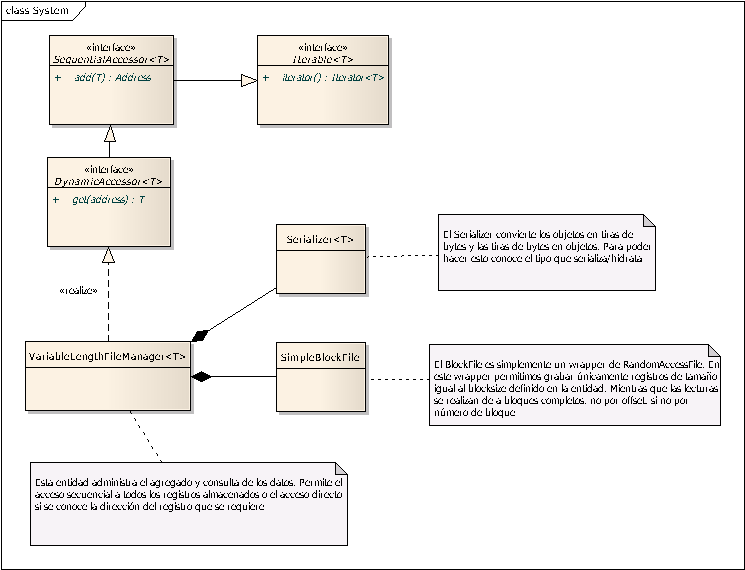
\includegraphics[scale=0.8]{img/ClassDiagramVariableLengthFileManager.png}
	\end{center}
	\caption{Probando la entrada estandar.} 
	\label{fig:classVLFM}
\end{figure}

\paragraph{}
El manejo de este archivo es simple, a medida que se le solicita agregar objetos los serializa con el serializador con que fue configurado y los agrega al �ltimo bloque (esto no significa que se escriba en este momento). Si se le solicita alg�n objeto en particular, mediante la direcci�n del mismo, este manejador de archivo accede al bloque que indique la direcci�n y mapea los datos del objeto correcto utilizando el mismo serializador.

\subsubsection[Operaci�n de creaci�n]{Agregado de registro}
El agregado de registros, como se mencion� anteriormente, primero serializa el objeto y luego lo agrega al �ltimo bloque. Este �ltimo bloque siempre se encuentra cacheado ya que se graba (o regraba) cuando esa cach�, de �ltimo bloque, desborda, es decir, su tama�o supera el tama�o designado para datos del bloque. En ese momento se graban todos los registros que estaban en cach� menos el �ltimo agregado. Si, este �ltimo agregado, tuviera un tama�o mayor al tama�o de designado para datos del bloque el mismo es dividido en n bloques y todos esos bloques son grabados.

\subsubsection[Operaci�n de lectura secuencial]{Lectura de todos los datos}
Se implement� un iterador de todo el archivo que comienza en el bloque cero, mapea todos los datos de ese bloque a objetos y los va devolviendo de a uno. Luego de devolver todos los de ese bloque, pasa al siguiente bloque y realiza la misma operatoria. Esto se repite hasta que no queden mas datos por hidratar. 

\subsubsection[Operaci�n de lectura aleatoria]{Lectura de un objeto dada una direcci�n}
El manejador de archivo lee el bloque desde el archivo f�sico (excepto que el mismo est� en cach�), y luego pasa los datos leidos por el serializador. Luego busca entre los objetos creados el que tenga la posici�n indicada por la direcci�n para poder devolverlo a qui�n se lo haya solicitado.

\subsection{Detalles t�cnicos}
Los bloques cuentan con la siguiente informaci�n de control. Los �ltimos 2 bytes indican (almacenado como un Short signado) la cantidad de registros enteros que posee el bloque (esto se utiliza al momento de hidratar, para no intentar hidratar mas registros de los que se encontraban almacenados), para el caso que el registro est� en m�ltiples bloques este valor se marca en cero y se toman los 8 bytes anteriores para indicar la posici�n del pr�ximo bloque que contiene datos del mismo registro.

Se implementaron 2 cach�s, muy b�sicas, la primera, ya fue mencionada, contiene el bloque actual donde se est�n agregando registros. La segunda contiene el �ltimo bloque leido del disco (para disminuir accesos a disco)


          % Manejadores de Archivos
\section{Buffers de Entrada y Salida}

El m�dulo de Buffers es quiz�s el mas sencillo de todos. Los buffers funcionan como una memoria de almacenamiento 
temporal de la informaci�n. Normalmente, se hace uso del buffer como una memoria intermedia, �til para almacenar 
informaci�n que est� por escribirse en un archivo o que haya sido le�do de uno.

Los buffers suelen mejorar el rendimiento en el intercambio de datos entre diferentes m�dulos de la aplicaci�n.

\subsection{An�lisis}

Los requisitos son claros: se necesita un Buffer de Entrada, del cual se leer�n los datos cargados del archivo, y un 
Buffer de Salida que ser� utilizado para escribir los datos que necesiten ser persistidos:

\begin{enumerate}
  \item \textsf{Buffer de Entrada}: Debe poder ser cargado con los datos que se lean de los archivos y permitir� 
    recuperar dichos datos para ser utilizados en la aplicaci�n.
  \item \textsf{Buffer de Salida}: Debe poder ser cargado con los datos que necesiten ser persistidos 
\end{enumerate}

\subsection{Soluci�n Propuesta}

texto
        % Buffers de Entrada y Salida
\section{Serializadores}
\label{sec:Serializadores}

El intercambio de datos con los archivos se realiza en forma de bytes (es decir, de una manera unificada) a traves de InputBuffer y OutputBuffer. Debe existir, entonces, una forma de "serializar" los datos hacia bytes y de poder recuperarlos luego a partir de ellos. Para lograrlo, esta serializaci�n debe incluir, adem�s de las conversiones a byte, los datos de control necesarios, tambi�n en forma de byte, para poder luego rearmar los objetos (datos) originales.
Para todo esto se defini� la interface Serializador con tres m�todos:
\begin{itemize}
\item dehydrate: Recibe un objeto a deshidratar y un OutputBuffer de destino. La implementaci�n debe convertir a una tira de byte el objeto recibido, incluyendo los datos y la informaci�n de control. Luego esa tira es informada al OutputBuffer.
\item hydrate: Recibe un InputBuffer del cual obtendr� una tira de bytes que usar� para armar un objeto. La tira de bytes que obtendr� desde el InputBuffer contiene los datos y la informaci�n de control necesaria para la hidrataci�n del objeto.
\item getDehydrateSize: Obtiene de manera r�pida (es decir, no realiza ninguna transformaci�n, solo el c�lculo) la cantidad de bytes que ocupar� el objeto deshidratado.
\end{itemize}

\begin{figure}[!htp]
	\begin{center}
		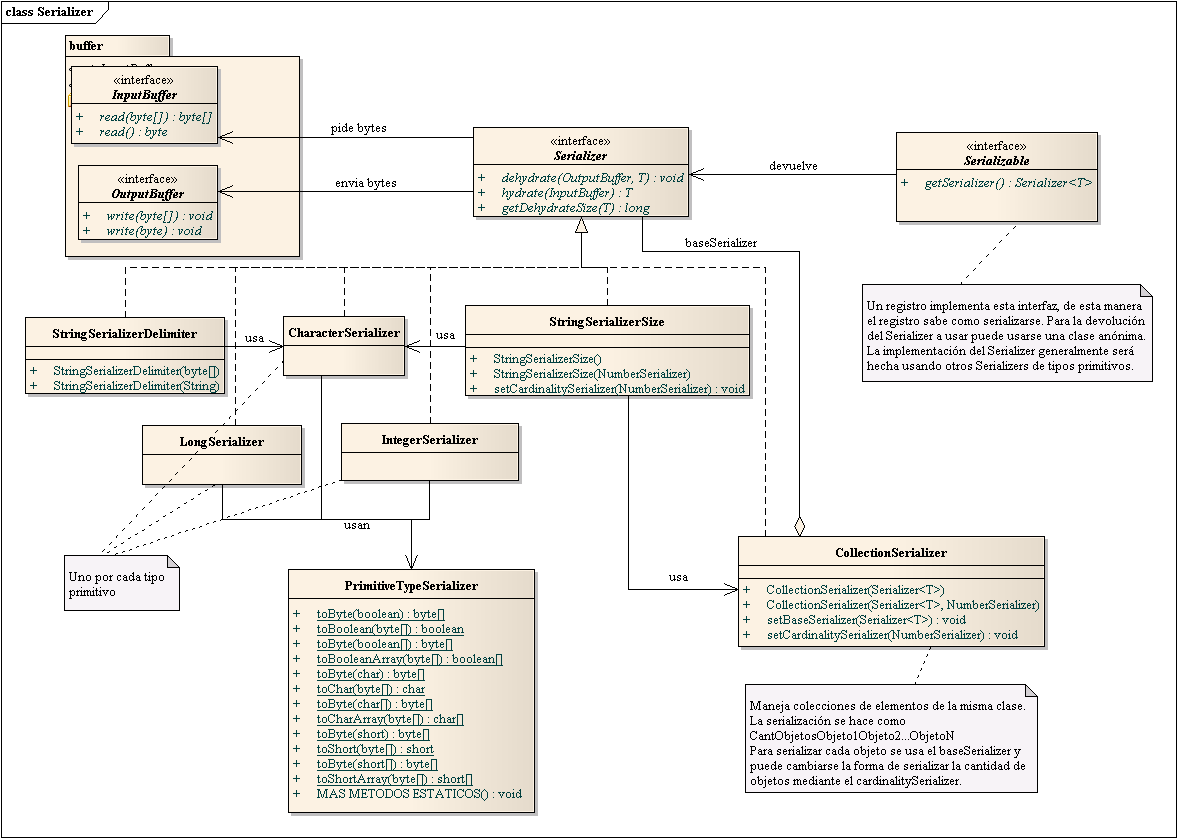
\includegraphics[scale=0.35,natwidth=1177pt, natheight=838pt]{img/Serializer.png}
	\end{center}
	\caption{Diagrama de clases del \textbf{Serializer}} 
\end{figure}

\subsection{Implementaciones}

Se definieron implementaciones de los tipos m�s comunes de datos a serializar:
\begin{itemize}
\item En principio la de tipos simples primitivos: usando el contrato definido por el equipo de Java en las interfaces DataInput y DataOutput, y su implementaci�n en RandomAccessFile como modelo, se definieron las operaciones de conversi�n entre tipos primitivos y tiras de bytes. Se defini� una clase con m�todos est�ticos para estas conversiones llamada PrimitiveTypeSerializer, y Serializadores para cada uno de los tipos primitivos que delegan su comportamiento en la clase mencionada.
\item Un serializador de colecciones para objetos de una clase que puedan ser serializados individualmente. La colecci�n ser� serializada como CantObjetosObjeto1...ObjetoN . Para la serializaci�n de cada objeto (1..N) se usa un serializador que parametriza de esa manera el serializador de colecciones. Por defecto la cantidad de objetos se serializa mediante el ShortSerializer, pero esto puede ser cambiado mediante el uso de un cardinalitySerializer diferente (y con esto variar la cantidad de bytes requerida para la serializaci�n de CantObjetos). Las cantidades se manejan como unsigned siempre. 
\item Serializadores de String. Se hicieron dos implementaciones:
\begin{itemize}
  \item La primera pone la cantidad de caracteres al principio y luego la serializaci�n de cada caracter. Para la implementaci�n se deleg� todo hacia un CollectionSerializer parametrizado con un CharacterSerializer y un ByteSerializer para la cantidad de caracteres (por tanto valen las mismas consideraciones de CollectionSerializer). El serializador de cantidad de caracteres puede ser intercambiado por otro.
  \item La segunda serializa cada caracter, apoy�ndose en CharacterSerializer, y pone una secuencia de bytes predeterminada (que puede ser intercambiada) al final de la tira de bytes.
\end{itemize}
\end{itemize}
\subsubsection{Uso con registros: Alternativas y soluci�n}

Un concepto con el que se trabaj� (y luego fue descartado) fue el de armar serializadores de manera din�mica:
Para ello pensamos en una clase llamada DynamicSerializer permit�a serializar colas de objetos de distintas clases. Se construye pasando un serializador base que ser� usado para serializar el primer elemento de la cola. Adem�s se recibe un serializador para el siguiente elemento que ser� englobado ("wrappeado") como un DynamicSerializer y devuelto (lo que permite usarlo estableci�ndole otro serializador como "siguiente", wrappeado y devuelto; as� con cada tipo de elemento de la cola). De esta manera cada DynamicSerializer realiza la serializaci�n de un elemento de la cola y delega la serializaci�n del resto al siguiente, repiti�ndose el proceso hasta el final.
De esta manera un objeto complejo, compuesto por varios elementos simples para los que existe un serializador, pueden ser serializados sin necesidad de crear una nueva clase/implementaci�n de serializer. Para ello primero deben tomarse los elementos simples que conforman el elemento compuesto y agregarlos a una cola en un orden preestablecido. Al hidratar debe tomarse la cola hidratada y tomando adecuadamente cada elemento de esta recomponer el objeto original. Es este armado/desarmado del elemento en la cola lo que nos llev� a abandonar est� opci�n pues, a pesar de quitar la necesidad de crear una clase por cada nuevo serializador, ensuciaba en muchos lados el c�digo por la necesidad de trabajar con la cola.

\begin{figure}[!htp]
	\begin{center}
		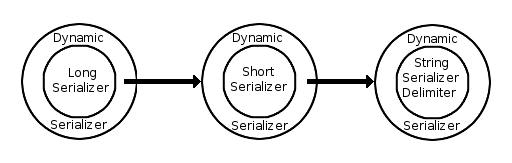
\includegraphics[scale=0.60,natwidth=512pt, natheight=163pt]{img/DynamicSerializerEjemplo.png}
	\end{center}
	\caption{Ejemplo de \textbf{DynamicSerializer}} 
\end{figure}

Fue entonces cuando se decidi� definir otra interfaz llamada Serializable que define un m�todo (getSerializer()) que permite conocer el serializador para un objeto en particular (el concepto ser�a "un serializable sabe como serializarse"). La implementaci�n del serializador puede hacerse en forma de una clase an�nima incluida en la clase a serializar dejando, entonces, el c�digo mucho m�s limpio.

Una alternativa para lograr la serializaci�n en forma din�mica era, usando como base la interface Serializer y sus implementaciones comunes, el uso de metadata a trav�s de annotations. La idea ser�a marcar, mediante una annotation creada especialmente, los atributos a serializar y el serializador (esto �ltimo [especificar el serializador] puede, incluso, ser opcional pu�s puede poseerse un Serializer por defecto para cada clase) a usar para dicho atributo. Dicho serializador puede ser uno de los de tipos primitivos mencionados m�s arriba (u otra implementaci�n de Serializer). Tambi�n debe marcarse -mediante la misma annotation- el orden de serializaci�n, es decir el orden que ocupar� cada atributo deshidratado en la tira de bytes (y entonces, el orden en que debe procesarse la tira para hidratarla). Por �ltimo habr� un Serializador especial, que recibe una clase parametrizada, capaz de interpretar la annotation mencionada para realizar la deshidrataci�n/rehidrataci�n de cualquier objeto que use use adecuadamente dicha annotation.
El problema con esta opci�n es que hace un uso intensivo de reflection, lo cual hace mucho m�s lento el proceso, por lo cual fue descartada.
    % Serializadores
\section{Servicios de Persistencia}

La persistencia ten�a como requerimiento t�cnico que los datos que maneja **The Speaker** fueran persistidos en dos archivos separados. En esta primera entrega el requerimiento era que fueran estrictamente dos archivos con la siguiente estructura l�gica definida.
\newcounter{archivo}
\begin{list}{\addtocounter{archivo}{1}\arabic{archivo}}
{
\setlength{\rightmargin}{\leftmargin}
}
\item \texttt{((palabra)i, offset)}
\item \texttt{(stream de audio)}
\end{list}
El primero est� compuesto de la dupla palabra (que es un identificador) y offset/referencia. Simbolizando que para la {\it palabra} el audio se encuentra en {\it referencia}.
El segundo archivo contiene los streams de audio capturados.

\subsection{An�lisis}
Lo primero que se observa de ambos archivos es que sus registros son de longitud variable y que hay homogeneidad en los datos a almacenar, es decir, que en cada archivo se almacenan siempre los mismos tipos de datos. De manera que, ambos archivos, a pesar de tener naturalezas de datos diferentes requieren el mismo manejo. Por lo cual, admiten una misma soluci�n de manejo del archivo mientras que la misma se mantenga indepen de la naturaleza de los datos a almacenar. 

Por otra parte, las operaciones que se deben permitir son el agregado de registros y la consulta de los mismos. El agregado de registros no requiere, en ninguno de los dos casos, que se haga con un orden espec�fico. Mientras que la recuperaci�n de los datos, por otra parte, en el primer archivo debe poder ser secuencial (ya que se necesitan poder acceder a cada una de las palabras) y en el segundo caso debe poder accederse directamente a un registro que conozco su posici�n dentro del archivo. Por lo cual, estamos ante una organizaci�n secuencial de acceso relativo. Pudiendo recorrerse tanto secuencialmente como acceder a un registro espec�fico (si se conoce previamente su direcci�n). La implementaci�n de esta funcionalidad se hizo en la clase  {\textbf{VariableLengthFileManager}.}

\subsection{Soluci�n propuesta}
Se utilizar� una entidad para abstraer a cada uno de los archivo, ambas entidades con el mismo comportamiento. Esta entidad se encarga permite tanto la carga de registros, como dos diferentes tipos de recuperaci�n de registros (completa y secuencial, o, de un �nico registro y direccionada). 
Para que la misma clase pueda persistir archivos con registros de diferente naturaleza se implementaron los serializadores  {\textit{(ver secci�n \ref{sec:Serializadores}.)}}

El serializador es configurado en cada archivo a manejar y realiza las dos conversiones necesarias: 
\begin{list}{+}{\setlength{\rightmargin}{\leftmargin}}
\item la tira de bytes leida en un objeto (Mapeo)
\item un objeto en una tira de bytes que ser� grabada (Serializaci�n)
\end{list}

El manejo de este archivo es simple, a medida que se le solicita agregar objetos los serializa con el serializador con que fue configurado y los agrega al �ltimo bloque (esto no significa que se escriba en este momento). Si se le solicita alg�n objeto en particular, mediante la direcci�n del mismo, este manejador de archivo accede al bloque que indique la direcci�n y mapea los datos del objeto correcto utilizando el mismo serializador.

\subsubsection[Operaci�n de creaci�n]{Agregado de registro}
El agregado de registros, como se mencion� anteriormente, primero serializa el objeto y luego lo agrega al �ltimo bloque. Este �ltimo bloque siempre se encuentra cacheado ya que se graba (o regraba) cuando esa cach�, de �ltimo bloque, desborda, es decir, su tama�o supera el tama�o designado para datos del bloque. En ese momento se graban todos los registros que estaban en cach� menos el �ltimo agregado. Si, este �ltimo agregado, tuviera un tama�o mayor al tama�o de designado para datos del bloque el mismo es dividido en n bloques y todos esos bloques son grabados.

\subsubsection[Operaci�n de lectura secuencial]{Lectura de todos los datos}
Se implement� un iterador de todo el archivo que comienza en el bloque cero, mapea todos los datos de ese bloque a objetos y los va devolviendo de a uno. Luego de devolver todos los de ese bloque, pasa al siguiente bloque y realiza la misma operatoria. Esto se repite hasta que no queden mas datos por hidratar. 

\subsubsection[Operaci�n de lectura aleatoria]{Lectura de un objeto dada una direcci�n}
El manejador de archivo lee el bloque desde el archivo f�sico (excepto que el mismo est� en cach�), y luego pasa los datos leidos por el serializador. Luego busca entre los objetos creados el que tenga la posici�n indicada por la direcci�n para poder devolverlo a qui�n se lo haya solicitado.

\subsection{Detalles t�cnicos}
Los bloques cuentan con la siguiente informaci�n de control. Los �ltimos 2 bytes indican (almacenado como un Short signado) la cantidad de registros enteros que posee el bloque (esto se utiliza al momento de hidratar, para no intentar hidratar mas registros de los que se encontraban almacenados), para el caso que el registro est� en m�ltiples bloques este valor se marca en cero y se toman los 8 bytes anteriores para indicar la posici�n del pr�ximo bloque que contiene datos del mismo registro.

Se implementaron 2 cach�s, muy b�sicas, la primera, ya fue mencionada, contiene el bloque actual donde se est�n agregando registros. La segunda contiene el �ltimo bloque leido del disco (para disminuir accesos a disco)


   % Servicios de Persistencia

\end{document}
